\cotefile{10}
\scanpage{33}
\mspage{\handwritten{1}}
% archive sheet number: 32

\uline{10. Passage à la limite projective dans les préschémas en groupes et les préschémas à groupe d'opérateurs.}

\margin{\handwritten{\figure{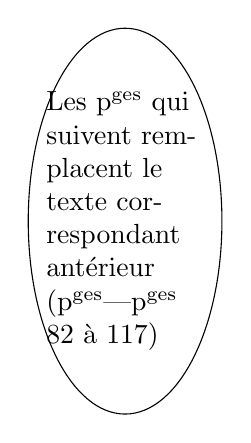
\begin{tikzpicture}
\node[text width=2cm,align=left,inner sep=2pt] at (0,0) {Les p\textsuperscript{ges} qui suivent remplacent le texte correspondant antérieur \unsure{(p\textsuperscript{ges}|p\textsuperscript{ges}} 82 à 117)};
\draw (0,0) ellipse (1.23 and 2.45);
\end{tikzpicture}}}}
\handwritten{10.}0. Rappelons le résultat essentiel de (EGA IV 8.8) : Etant donnée la situation suivante : $S_o$ un préschéma qu\handwritten{/}asi-compact et quasi-séparé, $I$ un ensemble préordonné filtrant croissant, $(\handwritten{\unsure{\mathscr{A}|\mathcal{A}}}_i)_{i\handwritten{\in}I}$ un système inductif de $\handwritten{\mathcal{O}}_{S_o}$-Algèbres commutatives quasi-cohérentes, $\handwritten{\mathscr{A}}=\underset{\handwritten{\longrightarrow}}{\lim}\handwritten{\mathscr{A}}_i$, $S_i=\operatorname{Spec}\handwritten{\mathscr{A}}_i$ pour $i\handwritten{\in}I$, et $S=\operatorname{Spec}\handwritten{\mathscr{A}}$, \handwritten{a}lors la catégorie des $S$-préschémas de présentation finie est déterminée à équivalence près par la donnée des catégories des $S_i$-préschémas de présentation finie, des foncteurs \inserted{entre ces catégories} $\handwritten{\rho}_{ij}:X_i\handwritten{\longmapsto}X_i\times_{S_i}S_j$ \deleted{\unsure{,}} pour $i\handwritten{\leqq}j$, et des isomorphismes de transitivité $\handwritten{\rho}_{jk}\mathbin{\unsure{o|\circ}}\handwritten{\rho}_{ij}\handwritten{\xrightarrow{\sim}\rho}_{ik}$. \deleted{Plus précisément,} \handwritten{Précisons.}

\margin{\handwritten{\figure{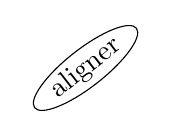
\begin{tikzpicture}
\node[rotate=38,inner sep=1pt] at (0,0) {aligner};
\draw[rotate=38] (0,0) ellipse (.82 and .24);
\end{tikzpicture}}\quad )\quad )}}
Etant donné $j\handwritten{\in}I$, et un $S_j$-préschéma de présentation finie $X_j$, nous poserons,pour tout $i\handwritten{\in}I$ tel que $j\handwritten{\leqq}i$, $X_i=X_j\handwritten{\times}_{S_j}S_i$, et $X=X_j\handwritten{\times}_{S_j}S$. Alors :\inserted{\handwritten{(EGA \uline{IV} 8.8.2)}}\handwritten{\unsure{;|:}}\margin{\handwritten{(}}

\uline{i) Etant donné $j\handwritten{\in}I$, et deux $S_j$-préschémas de présentation finie $X_j$ et $Y_j$, l'application canonique de $\underset{i\handwritten{\geqslant}j}{\underset{\handwritten{\longrightarrow}}{\lim}}\operatorname{Hom} S_i(X_i,Y_i)$ dans $\operatorname{Hom}(X,Y)$ est bijective}\margin{\handwritten{(}}

\uline{ii) Pour tout $S$-préschéma de présentation finie $X$, il existe un indice $j\handwritten{\in}I$, \deleted{et} un $S_j$-préschéma de présentation finie $X_j$ et un $S$-isomorphisme $X\handwritten{\xrightarrow{\sim}}X_j\handwritten{\times}_{S_j}S$.}

On en conclut (EGA IV 8.8.3) que, chaque fois qu'on aura un diagramme $D$ portant sur un nombre fini d'objets et de flèches de la catégorie des $S$-préschémas de présentation finie, on peut trouver un indice $i\handwritten{\in}I$ et un diagramme $D_i$ dans la catégorie des $S_i$-préschémas de présentation finie, tels que le diagramme $D$ provienne à isomorphisme près du diagramme $D_i$ par le changement de base $S\handwritten{\longrightarrow}S_i$. On peut même trouver $i$ et $D_i$ tels que tout carré cartésien de $D$ provienne d'un carré cartésien de $D_i$.

\handwritten{10.1.} De plus, un grand nombre de propriétés \deleted{de} courantes pour un morphisme, stables par changement de base, possèdent la propriété suivante ; étant donné un indice $j\handwritten{\in}I$ deux $S_j$-préschémas de présentation finie $X_j$ et $Y_j$ et un $S_j$-morphisme $u_j:X_j\handwritten{\longrightarrow}Y_j$, pour que $u=u_j\handwritten{\times}_{S_j}S$ ait la propriété $\handwritten{\mathbb{P}}$, il faut et il suffit qu'il existe un indice $i\handwritten{\in}I$ tel que $j\handwritten{\leqq}i$ et que $u_i=u_j\handwritten{\times}_{S_j}S_i$ ait la propriété $\handwritten{\mathbb{P}}$. Il en est ainsi dans le cas où $\handwritten{\mathbb{P}}$ est \deleted{la}\inserted{\handwritten{l'une des}} propriété\inserted{\handwritten{s}}\inserted{\handwritten{suivantes}} pour un morphisme:\deleted{\unsure{d'}}être séparé, surjectif, radiciel, affine, quasi-affine, fini, quasi-fini, propre, projectif, quasi-projectif, un isomor%
